\chapter{Калибровка атомно-зондового томографа ПАЗЛ-3D}\label{ch:ch3}

\section{Верификация точности восстановления 3Д координат}\label{sec:ch3/sect1}

\section{Определение зависимости качества данных от поляризации и мощности лазерного излучения}\label{sec:ch3/sect2}

Одной из критически важных характеристик пучка лазера для АЗТ является его поляризация относительно оси исследуемого образца. Известно, что плоскость колебаний вектора напряженности электрического поля пучка должна быть параллельна оси образца, в противном случае разрешение по массе становится крайне низким \cite{Houard10}. Чтобы убедиться в правильности выбранной плоскости поляризации, были проведены эксперименты с различным углом между плоскостью поляризации и осью образца. Отдельно необходимо отметить, что луч лазера перпендикулярен оси образца. Используемая лазерная система TETA 25ST фирмы Авеста-Проект позволяет устанавливать плоскость поляризации как раз в двух вариантах, в одном из которых плоскость поляризации параллельна оси образца, а в другом случае – перпендикулярна. Для демонстрации эффекта выбрана ДУО сталь Fe–13.5Cr–0.3Ti, имеющая выраженные пики двухзарядных изотопов Ni$^{2+}$ и Cr$^{2+}$ и пик Co$^{2+}$, расположенные вблизи основного пика $Fe_{56} ^{2+}$, которые в случае неоптимальных условий эксперимента будут неразличимы. Сбор данных проводился при следующих параметрах: частота воздействий лазера 25 кГц, мощность лазера 15 мВт, температура образца 50 К, скорость сбора данных 200 событий/с. Анализируемый набор данных – 300 тыс. событий для каждого из двух случаев поляризации (вдоль и поперек оси образца). Обработка данных проводилась специализированным программным обеспечением, разработанным в ИТЭФ. На Рисунке \cref{fig:Fe_Cr_polarization_a} показан масс-спектр, полученный при положении плоскости колебаний вектора напряженности электрического поля вдоль оси образца, а на Рисунке \cref{fig:Fe_Cr_polarization_b} – перпендикулярно оси образца. Как видно из Рисунков \cref{fig:Fe_Cr_polarization_a,fig:Fe_Cr_polarization_b}, поляризация лазера вносит существенный вклад в разрешение по массе – пики Cr, Ni и Co на масс-спектре с поляризацией вдоль оси образца отчетливо разрешаются, для основного пика железа $\frac{M}{\Delta M_{50\%}} = 620$ и $\frac{M}{\Delta M_{10\%}} = 210$, в отличие от случая с поляризацией перпендикулярно оси образца, где $\frac{M}{\Delta M_{50\%}} = 100$ и $\frac{M}{\Delta M_{10\%}} = 10$.

\begin{figure}[htb]
	\centerfloat{
		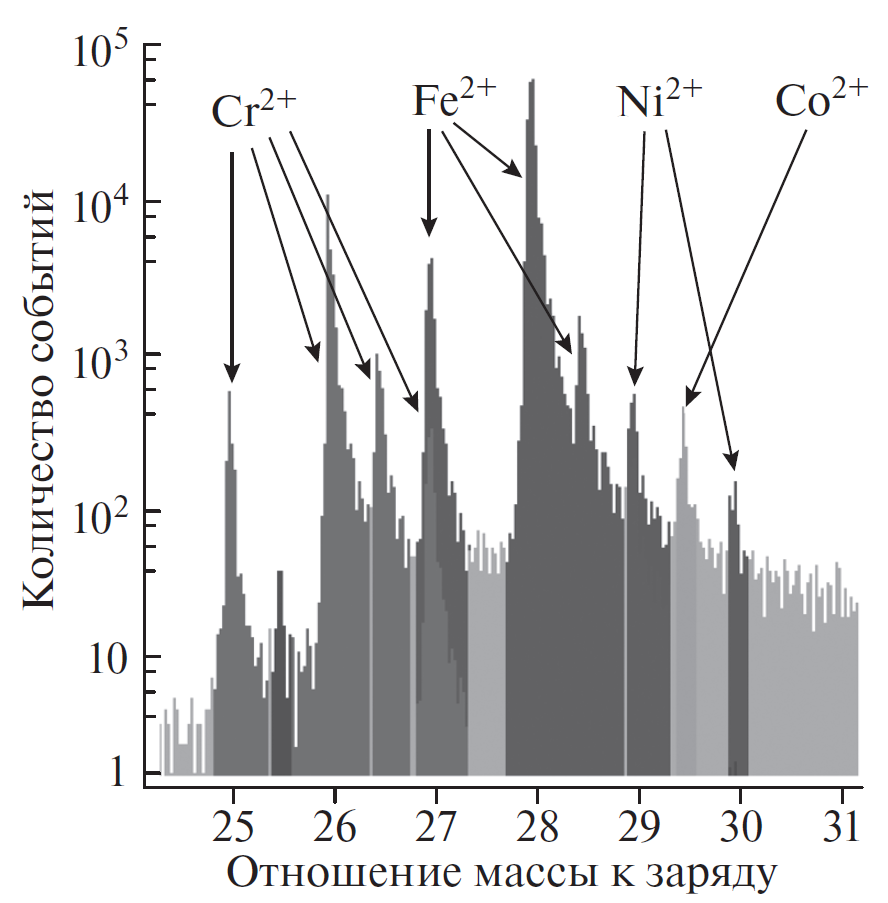
\includegraphics[width=\textwidth]{Fe_Cr_polarization_a}
	}
	\caption{Масс-спектр, полученный при поляризации лазера вдоль оси образца}
	\label{fig:Fe_Cr_polarization_a}
\end{figure}
\begin{figure}[htb]
	\centerfloat{
		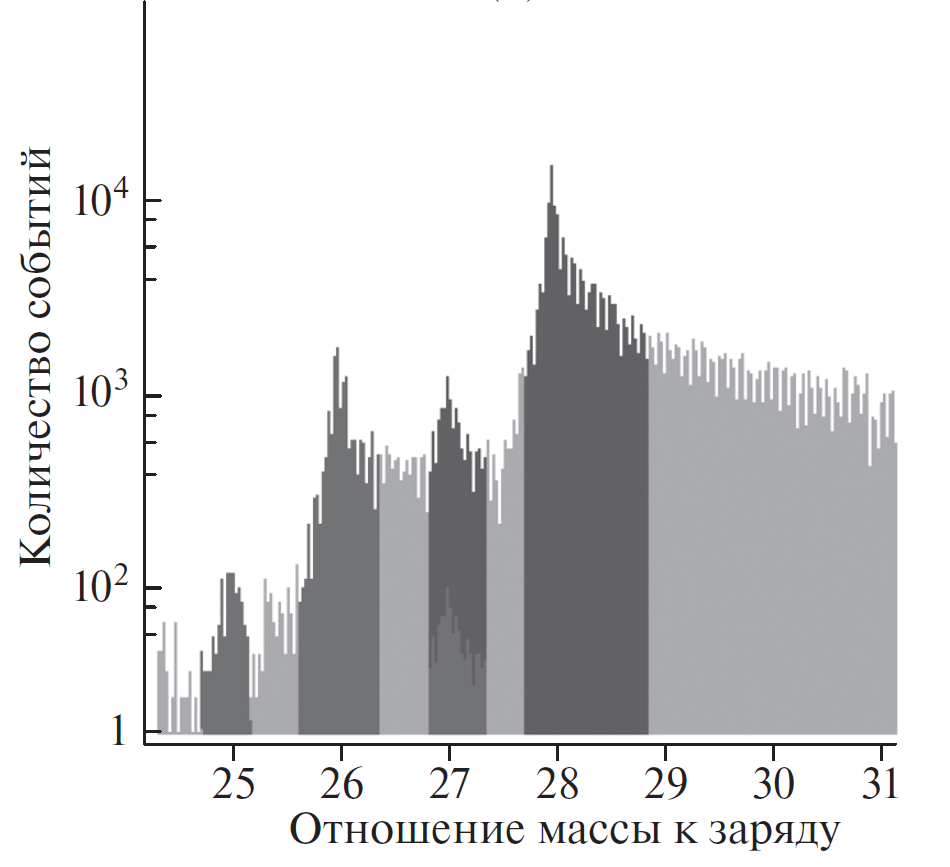
\includegraphics[width=\textwidth]{Fe_Cr_polarization_b}
	}
	\caption{Масс-спектр, полученный при поляризации лазера перпендикулярно оси образца}
	\label{fig:Fe_Cr_polarization_b}
\end{figure}


Другой основной варьируемый параметр прибора, который требует точной подстройки в процессе проведения анализа образцов, является мощность лазера. Мощность лазера способна влиять на ряд параметров точности восстановления данных, в частности на качество получаемого масс-спектра. Для исследования качества получаемого масс-спектра в зависимости от используемой мощности лазера, был использован модельный бинарный сплав Fe–Cr (22 ат. \%). Сбор данных проводился при эквивалентных описанному выше условиях. На Рисунке \cref{fig:Fe_Cr_power} представлен масс-спектр, полученный при мощности лазера 1 мВт. Как видно, химическая идентификация при столь малой мощности невозможна из-за случайного испарения атомов, не связанного с воздействием лазера.

\begin{figure}[htb]
	\begin{minipage}[b]{0.49\textwidth}\centering
		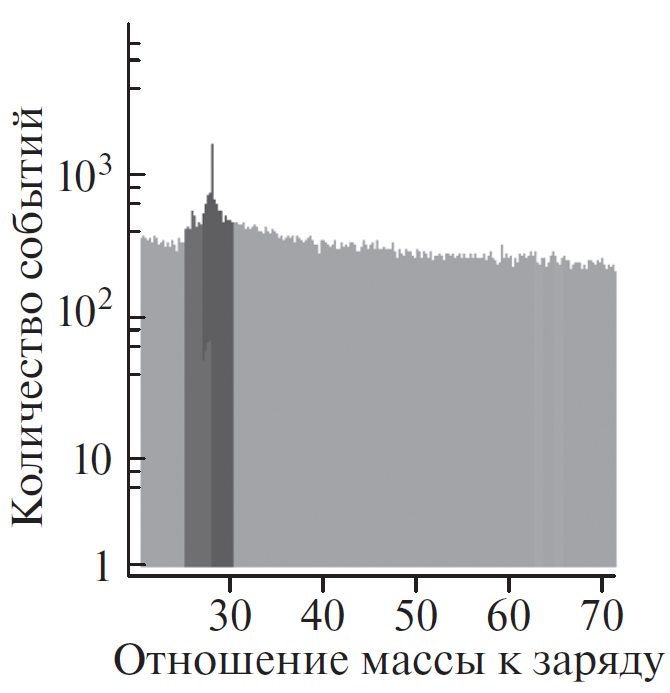
\includegraphics[width=\textwidth]{Fe_Cr_power_a} \\ а)
	\end{minipage}
	\begin{minipage}[b]{0.49\textwidth}\centering
		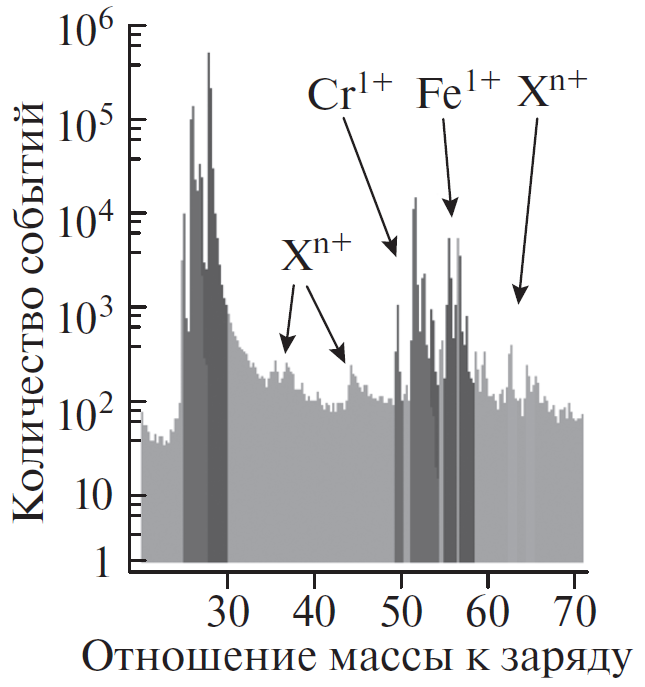
\includegraphics[width=\textwidth]{Fe_Cr_power_b} \\ б)
	\end{minipage}
	\begin{minipage}[b]{0.49\textwidth}\centering
		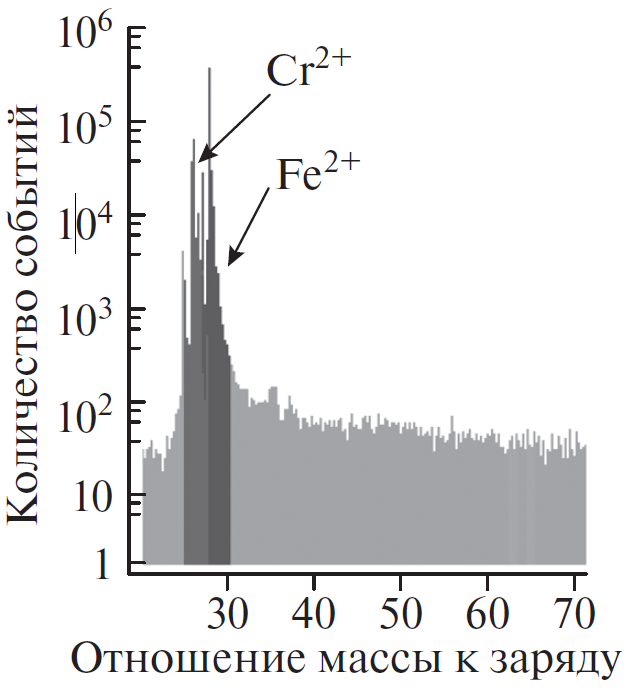
\includegraphics[width=\textwidth]{Fe_Cr_power_c} \\ в)
	\end{minipage}
	\caption{Примеры масс-спектров, полученных при различной мощности лазера: (а) при мощности 1 мВт; (б) при мощности 40 мВт (X$^{n+}$ – многозарядные и комплексные ионы); (в) при мощности 15 мВт.}
	\label{fig:Fe_Cr_power}
\end{figure}

При слишком высокой мощности лазера (более 40 мВт), пики разрешаются достаточно хорошо, однако происходит испарение большого количества многозарядных и сложных ионов (в том числе гидридов CrH, FeH), что затрудняет химическую идентификацию (см. Рисунок \cref{fig:Fe_Cr_power}). Этот эффект известен в атомно-зондовой томографии и связан с увеличением вероятности испарения некоторых элементов и их соединений при возрастании мощности воздействующего лазерного излучения \cite{Tu15}. К тому же при высокой мощности лазера происходит перегрев поверхности образца, что снижает пространственное разрешение \cite{Cerezo07}. При оптимальной мощности лазера (10–20 мВт) происходит испарение простых ионов, с наименьшим полем испарения, вследствие чего расшифровка масс-спектра наименее затруднительна, а также минимален шум от случайного испарения атомов (см. Рисунок \cref{fig:Fe_Cr_power}). Разрешение по массе для основного пика железа в этом случае составило $\sim$520.


\FloatBarrier
Заключение ррр рррр

\section{Определение оптимальных параметров испарения для сплава Al-Cu-Mn-Sn}\label{sec:ch3/sect3}



\FloatBarrier

\section{Сравнение атомно-зондовых данных для установок ПАЗЛ-3D и ECOTAP на примере сплава Al-Cu-Zr}\label{sec:ch3/sect4}

Модернизированная АЗТ установка АТЛАЗ была собрана на базе прибора CAMECA ECOTAP. Позиционно-чувствительный детектор DLD~120 с эффективностью детектирования 60~$\%$ и диаметром чувствительной части 120~мм фирмы RoentDek Handels GmbH установлен вместо системы автоионной микроскопии. Лазерная система испарения основана на пикосекундном лазере Huaray Olive-532-15 с длительностью лазерных импульсов менее 10 пс, длиной волны излучения 532 нм, частотой повторения импульсов до 1~МГц и максимальной энергией импульса не менее 15~мкДж на всем диапазоне частот. Для поддержания высокого напряжения на исследуемом образце использован штатный высоковольтный источник постоянного напряжения установки ECOTAP: BERTAN205B-20R фирмы Spellman High Voltage Electronics Corporation. В качестве системы охлаждения образца использована штатная система установки ECOTAP на основе системы Cryodyne 350 CP фирмы CTI Cryogenics. Позиционирование лазерного луча проводится при помощи диэлектрического зеркала диаметром 2", установленного в оправу, приводимую в движение актуаторами PIAK10 фирмы Thorlabs. Процесс наведения контролируется при помощи камеры Basler acA2440-35um. Установка АТЛАС использует прямопролетную геометрию испарения образца с расстоянием от образца до детектора 265~мм.

В установке ПАЗЛ-3D \cite{scbibAPPLE} также используется детектирующая система фирмы RoentDek Handels
GmbH. Данная система отличается эффективностью детектирования в 80–90 $\%$ и диаметром детектора 80 мм, в то время как у АТЛАЗ – 120 мм. Для испарения установлена лазерная система испарения TETA-25ST производства ООО~“Авеста”. В проведенных исследованиях \cite{scbibAPPLE,Shutov18} была оценена точность восстановления данных: пространственное разрешение не хуже 4 \r{A}, разрешение по массе на полувысоте 500-600 отн. ед. Установка ПАЗЛ-3D также использует прямопролетную геометрию испарения образца с расстоянием между образцом и детектором 183 мм. 
Для исследования выбирались материалы, хорошо изученные группой НИЦ “Курчатовский Институт”, содержащие наноразмерные кластеры. Из конструкционных сталей была выбрана сталь 16Х12МВСФБР ЭП-823 \cite{Porollo04} после облучения ионами (далее ЭП-823), так как в ней присутствуют кластеры с достаточно высокой плотностью. В классе алюминиевых сплавов – Al-3.3Cu-2.5Mn-0.5Zr (мас. \%) после отжига при 350 и 450°С \cite{Belov22,Belov21} (далее Al-Cu-Mn-Zr 350°С и Al-Cu-Mn-Zr 450°С соответственно). Также проведено сравнение полученных данных при исследовании вольфрама чистотой 99.95~\% для подтверждения пространственного разрешения АТЛАЗ. Погрешности для концентраций рассчитаны по формуле, представленной в работе \cite{Danoix071,Danoix072}. В случае, когда на одно состояние приходилось более одного исследования, в качестве погрешности указано среднее отклонение от среднего значения.
Критериями сравнения точности восстановления данных были выбраны следующие характеристики: разрешение по массе на полувысоте пика, разрешение по массе на 10~\% высоты пика точность определения концентраций матрицы и частиц, точность определения размеров частиц. Также использовались технические параметры для сравнения данных. Как показано в работах \cite{Tang10,Geuser07} одним из важнейших таких параметров можно считать количество и распределение мульти-событий. Для исследуемых объемов рассчитаны как общий процент мульти-событий, так и доля мульти-событий, приходящаяся на элементы, которые является кластеро-/фазо-образующими. Помимо мульти-событий, учитывались величины скорости детектирования, уровень шума и соотношение детектируемых ионов разных степеней ионизации для основного химического элемента.

Образцы приготовлены с помощью электрохимического утонения. Все данные на ПАЗЛ-3D и АТЛАЗ собраны при температуре образца 50~К. Мощность лазера составляла на ПАЗЛ-3D 85 $\pm$ 1 мВт и на АТЛАЗ 3 $\pm$ 0.5 мВт. Скорость сбора данных представлена ниже в таблице. Восстановление и обработка данных проводилась в ПО КВАНТМ-3D. Параметры восстановления для ПАЗЛ-3D были выбраны следующие: полевой множитель kf от 4 до 6, множитель сжатия изображения ICF от 1.2 до 1.6. Атомные карты представлены на Рисунке.  \cref{fig:APPLEvsATLAS}. Алгоритмы восстановления масс-спектра и 3D данных использовались те же, что и для вольфрама. Для определения состава включений Zr для сплава Al-Cu-Mn-Zr 350 °C, ввиду их не сферичной формы, использовались изоконцентрационные поверхности. Ниже, в Таблицах \cref{tab:paramsAPPLEvsATLAS,tab:matrixAPPLEvsATLAS,tab:clustersAPPLEvsATLAS}, представлено сравнение данных для разных установок для алюминиевого сплава.

\begin{table} [htbp]
	\centering
	\caption{Сравнение характеристик точности восстановления данных для алюминиевых сплавов Al-Cu-Mn-Zr}
	\label{tab:paramsAPPLEvsATLAS}
	\begin{SingleSpace}
		\begin{tabular} {| c | c | c | c | c |}
			\hline
			    {} & \thead{ПАЗЛ-3D, \\350 \textdegree C} & \thead{АТЛАЗ, \\350 \textdegree C} & \thead{ПАЗЛ-3D, \\450 \textdegree C} & \thead{АТЛАЗ, \\450 \textdegree C} \\ \hline
			$M/\Delta M_{50\%}$ Al$^+$ & 670  & 260  & 421  & 430               \\ \hline
			$M/\Delta M_{10\%}$ Al$^+$ & 206  & 120  & 146  & 190               \\ \hline
			Мульти-события, \%         & 0.7  & 2.9  & 0.9  & 2.9               \\ \hline
			Мульти-события Cu, \%      & 4.23 & 0.54 & 7.11 & 3.17              \\ \hline
			Мульти-события Zr, \%      & 7.31 & 0.85 & 0.18 & 0.6               \\ \hline
			Шум, 10$^{-5}$ отн. ед. & 5.4   & 1.9   & 10.7  & 1.67  \\ \hline
			Скорость сбора данных, атомов/возд.        & 0.005 & 0.006 & 0.007 & 0.007 \\ \hline
			Соотношение Al$^+$/Al$^{++}$, отн. ед.    & 640   & 310   & 630   & 450   \\ \hline
		\end{tabular}
	\end{SingleSpace}
\end{table}

Для Al-Cu-Mn-Zr 450 °С на ПАЗЛ-3D представлены средние значения характеристик данных по трем исследованным образцам. Проведено сравнение химического состава материалов как в кластерах для Al-Cu-Mn-Zr 350 °С, так и в матрице для Al-Cu-Mn-Zr 350 °С и 450 °С. Ввиду не сферичной формы включений Zr была использована методика изо-концентра ционных поверхностей (поверхностей одинаковой концентрации). Для определений границ включений были построены поверхности так, чтобы перегиб профиля концентраций, построенный нормально к поверхности (проксиграмма) проходил точно на полувысоте по концентрациям \cite{Hellman07}. Параметры, используемые для построения и расчетов, были выбраны следующие: размер сетки 1-1.5 нм, делокализация 2 нм, изо-концентрация поверхности по 1.5 \% Zr. 

\begin{table} [htbp]
	\centering
	\caption{Состав кластеров [ат. \%] в алюминиевом сплаве Al-Cu-Mn-Zr после отжига при 350~°С, полученный
		на установках ПАЗЛ-3D и АТЛАЗ}
	\label{tab:matrixAPPLEvsATLAS}
	\begin{SingleSpace}
		\begin{tabular} {| c | c | c |}
			\hline
			{} & ПАЗЛ-3D & АТЛАЗ \\ \hline
			Al       & 96.9 $\pm$ 0.3  & 99.7 $\pm$ 0.4   \\ \hline
			Cu       & 0.3 $\pm$ 0.1   & 0.3 $\pm$ 0.1    \\ \hline
			Mn       & 0.04 $\pm$ 0.02 & 0.003 $\pm$ 0.002  \\ \hline
			Zr       & 2.4 $\pm$ 0.3   & 2.8 $\pm$ 0.2    \\ \hline
			Ni, C, O & Баланс & Баланс   \\ \hline			
		\end{tabular}
	\end{SingleSpace}
\end{table}

\begin{figure}[h!tb]
	\begin{minipage}[b][][b]{0.49\textwidth}\centering
		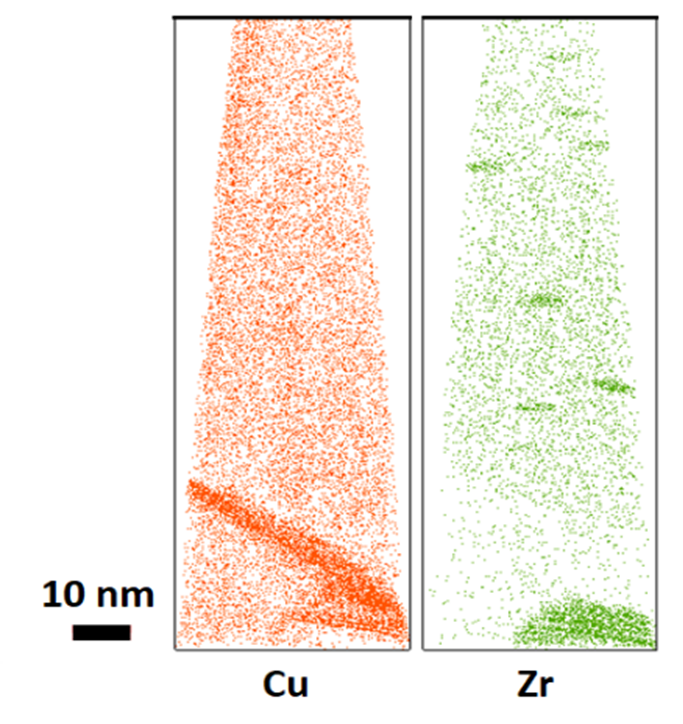
\includegraphics[scale=0.5]{APPLEvsATLAS_apple} \\ а)
	\end{minipage}
	%\hfill
	\begin{minipage}[b][][b]{0.49\textwidth}\centering
		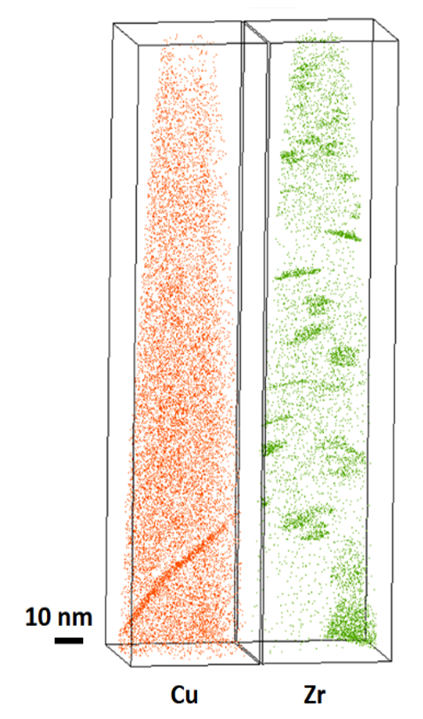
\includegraphics[scale=0.8]{APPLEvsATLAS_atlas} \\ б)
	\end{minipage}
	\caption{а) Атомные карты сплава Al-Cu-Mn-Zr 350°С ПАЗЛ-3D. б) Атомные карты сплава Al-Cu-Mn-Zr 350°С АТЛАЗ.}
	\label{fig:APPLEvsATLAS}
\end{figure} 

Данные для Al-Cu-Mn-Zr 450°С на ПАЗЛ-3D рассчитаны как среднее по трем исследованным образцам, погрешности также для данного материла рассчитаны как среднее отклонение от среднего значения. Плотность включений для данных с ПАЗЛ-3D составила (0.9 $\pm$ 0.1) x 10$^{23}$ и (1.40 $\pm$ 0.05) x 10$^{23}$ штук в м$^3$ для АТЛАЗ.

Исследование ЭП-823
Условия сбора данных были во много идентичны тем, что использовались при исследовании алюминиевых сплавов. Температура образцов составляла 50~К, мощность лазера на ПАЗЛ-3D 40 $\pm$ 1 мВт, на АТЛАЗ 2 $\pm$ 0.5 мВт. Для восстановления атомно-зондовых данных и их обработки также использовалось ПО КВАНТМ~3D и те же алгоритмы 3D восстановления. Множитель поля $k_f$ составлял 4.5, коэффициент сжатия изображения ICF от 1.2 до 1.35. Процесс обработки масс-спектра включал в себя первоначальную разметку с помощью автоматизированного инструмента разметки модуля “environment editor”, после была проведена ручная коррекция размеченных пиков. Далее был проведен пересчет пресекающихся пиков, в частности для Cr и Fe, ориентируясь на соседние пики этих элементов. Был проведен пересчет коэффициента Ni++ с целью минимизировать влияние термического хвоста Fe. Пики меди были разделены и рассмотрены на 3D модели, с целью убедиться, что оба пика соответствуют Cu. Также были проверены пики Mo на возможное пересечение с Cr+. В образце на ПАЗЛ-3D, был обнаружен пик Nb между пиками Mo, на АТЛАЗ из-за повышенного шума этот пик не виден на масс-спектре. На Рисунке \cref{fig:APPLEvsATLAS_EP} показаны атомные карты объемов.

\begin{figure}[h!tb]
	\begin{minipage}[b][][b]{0.49\textwidth}\centering
		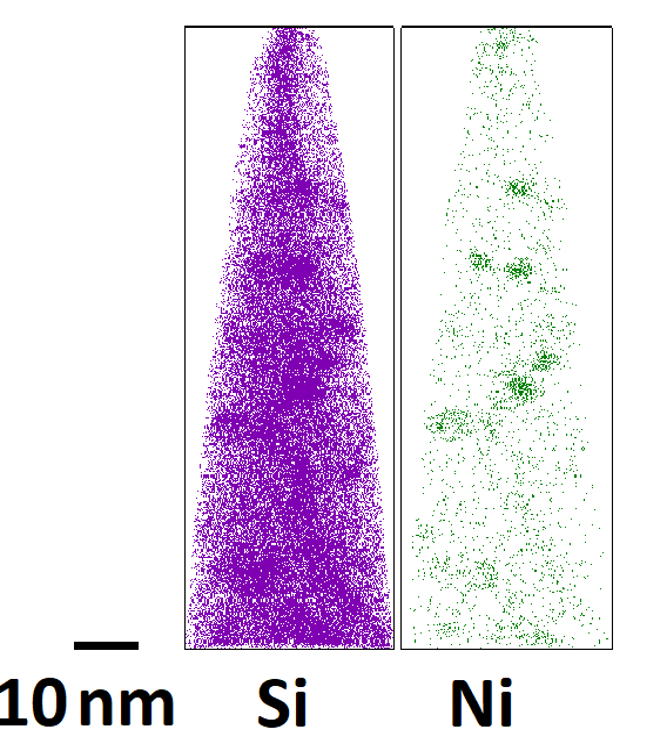
\includegraphics[scale=0.5]{APPLEvsATLAS_apple_EP} \\ а)
	\end{minipage}
	%\hfill
	\begin{minipage}[b][][b]{0.49\textwidth}\centering
		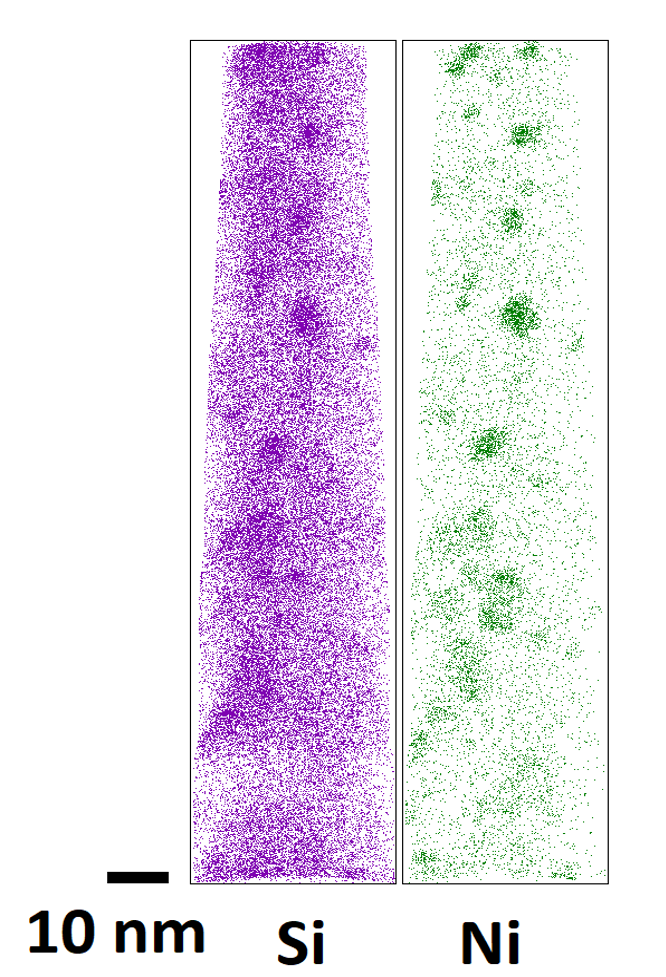
\includegraphics[scale=0.8]{APPLEvsATLAS_atlas_EP} \\ б)
	\end{minipage}
	\caption{Атомные карты облученной стали ЭП-823 на ПАЗЛ-3D (а) и АТАЛАЗ (б).}
	\label{fig:APPLEvsATLAS_EP}
\end{figure} 

Поиск кластеров был проведен по Ni+ согласно алгоритму максимального разделения [ссылка на максимальное разделение]. Из пересечения соответствующих графиков, получены параметры идентификации кластеров по методу максимальной сепарации ($N_min$ = 7 и R = 8 для ПАЗЛ-3D и $N_min$ = 7 и R = 7.5 для АТЛАЗ). По найденным параметрам были выделены кластеры, после их отделения от матрицы. Были просмотрены кластеры на 3D изображении для выявления случайного объединения или выделения несоответствующий области в качестве кластера. Был создан отдельный масс-спектр для кластеров. В этом масс-спектре учитывались в приоритете элементы обогащения, в частности Ni++. Также внутри кластеров для обеих установок был обнаружен Nb и, соответственно, размечен. Данные масс-спектра отдельно матрицы и кластеров были экспортированы и объединены в общей таблице. В Таблицах \cref{tab:paramsAPPLEvsATLAS_EP3,tab:matrix_clustersAPPLEvsATLAS}, представлено сравнение данных для разных установок отдельно для стали ЭП-823.

\begin{table} [htbp]
	\centering
	\caption{Сравнения характеристик точности восстановления данных для ЭП-823 на установках ПАЗЛ-3D и АТЛАЗ}
	\label{tab:paramsAPPLEvsATLAS_EP3}
	\begin{SingleSpace}
		\begin{tabular} {| c | c | c |}
			\hline
			{}                                     & ПАЗЛ-3D & АТЛАЗ   \\ \hline
			$M/\Delta M_{50\%}$ Al$^+$             & 938     & 726     \\ \hline
			$M/\Delta M_{10\%}$ Al$^+$             & 245     & 329     \\ \hline
			Мульти-события, \%                     & 1.4     & 17.7                 \\ \hline
			Мульти-события Ni, \%                  & 1.7     & 28.6             \\ \hline
			Мульти-события Si, \%                  & 0.4     & 26.1             \\ \hline
			Мульти-события Cu, \%                  & 3.9     & 6.7             \\ \hline
			Шум, 10$^{-5}$ отн. ед.                & 10.05   & 30.1     \\ \hline
			Скорость сбора данных, атомов/возд.    & 0.008   & 0.01  \\ \hline
			Соотношение Al$^+$/Al$^{++}$, отн. ед. & 307     & 368     \\ \hline
		\end{tabular}
	\end{SingleSpace}
\end{table}

\begin{table} [htbp]
	\centering
	\caption{Сравнение состава матрицы [ат. \%] для алюминиевых сплавов Al-Cu-Mn-Zr после отжига при температурах 350 °С и 450 °С, полученных на установках ПАЗЛ-3D и АТЛАЗ}
	\label{tab:matrix_clustersAPPLEvsATLAS}
	\begin{SingleSpace}
		\begin{tabular} {| c | c | c | c | c |}
			\hline
			{} & \thead{ПАЗЛ-3D матрица} & \thead{АТЛАЗ матрица} & \thead{ПАЗЛ-3D кластеры} & \thead{АТЛАЗ кластеры} \\ \hline
			Fe       & 83.43 $\pm$ 0.02 & 83.98 $\pm$ 0.02  & 48 $\pm$ 1      & 53 $\pm$ 1  \\ \hline
			Cr       & 11.11 $\pm$ 0.06 & 10.51 $\pm$ 0.05  & 6.9 $\pm$ 0.8   & 7.3 $\pm$ 0.7   \\ \hline
			Si       & 2.59 $\pm$ 0.06  & 1.88 $\pm$ 0.05   & 15 $\pm$ 1      & 10.0 $\pm$ 0.8 \\ \hline
			Mn       & 0.94 $\pm$ 0.06  & 1.98 $\pm$ 0.05   & 4.5 $\pm$ 0,6   & 4.7 $\pm$ 0.5   \\ \hline
			Ni       & 0.59 $\pm$ 0.06  & 0.78 $\pm$ 0.05   & 23 $\pm$ 1      & 21 $\pm$ 1   \\ \hline
			Cu       & 0.05 $\pm$ 0.04  & 0.08 $\pm$ 0.05   & 0.2 $\pm$ 0,1   & 0.5 $\pm$ 0.2   \\ \hline
			W        & 0.16 $\pm$ 0.06  & 0.28 $\pm$ 0.05   & 0.03 $\pm$ 0,03 & 0.2 $\pm$ 0.1   \\ \hline
			C        & 0.08 $\pm$ 0.06  & 0.09 $\pm$ 0.05   & 0.11 $\pm$ 0,06 & 0.08 $\pm$ 0.06   \\ \hline
			Nb       & 0.07 $\pm$ 0.06  & -                 & 0.3 $\pm$ 0.1   & 0.5 $\pm$ 0.1   \\ \hline
			Остальные & Баланс & Баланс & Баланс & Баланс               \\ \hline			
		\end{tabular}
	\end{SingleSpace}
\end{table}


В Таблице \cref{tab:matrix_clustersAPPLEvsATLAS} представлено сравнение химического состава материалов как в кластерах, так и в матрице для стали ЭП-823. Средний размер кластеров на ПАЗЛ-3D составил (2.8 $\pm$ 0.2) нм, на АТЛАЗ средний размер равен (3.2 $\pm$ 0.4) нм. Рассчитана средняя плотность кластеров в объеме, которая составила (1.2 $\pm$ 0.4) x 10$^{23}$ и (1.1 $\pm$ 0.2) x 10$^{23}$ м$^3$ для ПАЗЛ-3D и АТЛАЗ соответственно.

Как видно из полученных выше характеристик точности восстановления данных установки ПАЗЛ-3D и АТЛАЗ сравнимы по разрешению по массе и для алюминиевых сплавов, и для сталей. Сравнение количества шума проводилось на участках масс-спектра после пиков основных элементов и сопоставлялось с учетом нормирования на общее число собранных атомов. Количество шума при исследовании алюминиевого сплава отличается в 3-6 раз в пользу АТЛАЗ, но в случае со сталью ситуация противоположная (на АТЛАЗ шума больше в три раза). Данный факт вызван скорее разными условиями испарения образцов – разная скорость сбора данных и неодинаковая форма образцов. Наблюдаются общие закономерности при сравнении доли мульти-событий. На АТЛАЗ детектируется существенно больше мульти-событий, чем на ПАЗЛ-3D. В случае исследования чистых материалов или алюминиевых сплавов это практически не играет роли. При исследовании стали получены данные с 17.7 \% мульти-событий. Предположительно, это может быть вызвано использованием криогенной системы без устройств гашения вибраций на АТЛАЗ (вибрации могут составлять более 20 мкм), на которую непосредственно закреплен держатель образца. Это может приводить к частому выходу образца из области освещения лучом лазера, что влечет за собой необходимость поддерживать более высокую интенсивность испарения в моменты корректного освещения вершины образца. Известно, что в этом случае количество мульти-событий возрастает, и снижается точность химической идентификации \cite{scbibOptParamsYAFI}. Различия в пропорции между элементами в мульти-событиях для алюминиевых сплавов, как видно из результатов, не вносит существенного различия в определяемый химический состав матрицы и кластеров. Скорее всего, отсутствие разницы обусловлено малым значением общего числа мульти-событий. Для ЭП-823, при исследовании на АТЛАЗ, получены существенно большие значения мульти-событий как для общее числа, так в пропорциях по элементам. Как следствие, наблюдаются отличия по концентрациям для Si, Mn, W и Cr, что, скорее всего, может быть нивелировано более точным подбором условий испарения или модернизацией прибора за счет уменьшения вибраций держателя образца.
Сравнение результатов исследования вольфрама позволяет заключить, что установки имеют практически идентичное пространственное разрешение 1-4 \r{A}. Это позволяет предположить, что все пространственные характеристики при сравнении данных должны быть иметь мало различий между установками. Данный тезис подтверждается при сравнении среднего размера кластеров в стали ЭП-823 и преципитатов Zr в алюминиевом сплаве. В обоих случаях средний размер нано-размерных объектов совпадает в пределах статистической погрешности. С другой стороны, в сплаве Al-Cu-Mn-Zr 350°С на разных установках наблюдается некоторое отличие рассчитанной плотности кластеров. Ввиду небольшой разницы результатов (всего в 1.5 раза) можно предположить, что причина отклонения в плотности частиц связана с реальными различиями плотности в разных зернах материала. При этом химический состав как матрицы, так и частиц для алюминиевых сплавов совпадает в пределах погрешности.

\FloatBarrier
\clearpage %чтобы картинки не уезжали в другие главы
\section{Методика коррекции 3Д восстановления атомно-зондовых данных с учетом атомной плотности}\label{sec:ch3/sect5}

Точность восстановления данных существенно зависит от параметров калибровки АЗТ и типа алгоритма восстановления. Трехмерные координаты вычисляются по известному принципу проекции. Можно использовать несколько алгоритмов восстановления координат. Основное различие между ними заключается в том, как они учитывают детали эволюции радиуса наконечника образца или координаты Z во время исследования APT \cite{Vurpillot16}. В наиболее распространенном алгоритме, предложенном Басом и др. \cite{Bas95}, предполагается, что радиус острия образца пропорционален напряжению. Этот алгоритм удобен для учета изменения формы образца и его радиуса. Однако это может быть неточно при анализе многофазного материала. Другой алгоритм, предложенный группами Blavette и Virpillot \cite{Vurpillot11,Gault11}, подходит для постоянного изменения угла зрения во время исследования АЗТ. Этот алгоритм хорошо подходит для восстановления распределения атомов в материалах с разными фазами. Однако он не работает, когда атомы фаз имеют значительно разные скорости испарения, и поэтому скорости изменения радиуса сильно различаются в разных фазах. Другой вариант состоит в том, что изменение радиуса может быть учтено с помощью его прямых измерений на изображении образца с помощью просвечивающей электронной микроскопии и электронного микроскопа \cite{Larson11}. Основными параметрами восстановления являются коэффициент сжатия изображения (ICF или $\xi$), длина полета иона, поле испарения для конкретного материала, коэффициент поля ($k_f$), атомный объем ($\Omega$), эффективность обнаружения и анализируемая область. Некоторые параметры, такие как эффективность обнаружения или анализируемая область, являются характеристиками АЗТ-устройства и не изменяются во время АЗТ-исследования. Однако другие параметры не постоянны. Например, ICF зависит от формы образца или электростатической системы \cite{Geiser09,Gipson08}. Для определения характера изменения этих параметров были проведены калибровочные исследования для различных типов АЗТ: ECOTAP \cite{Geiser09}, LAWATAP \cite{Renaud03}, LEAP 3000 \cite{Renaud06}. Также было проведено моделирование полевого испарения для определения зависимости параметров реконструкции от различных условий испарения \cite{Vurpillot11,Miller14,Hatzoglou19}. Следовательно, алгоритм трехмерной реконструкции, предложенный Басом и др., необходимо модифицировать. В методике восстановления АЗТ, основанной на алгоритме, предложенном Басом и др. \cite{Bas95}, радиус кривизны острия образца R определяется напряжением U, приложенным к образцу. Для восстановления поперечных координат (X, Y) атомов используется стереографическая проекция:

\begin{equation}
	\label{eq:equation3_1}
	X = R \sin{\phi}\sin{\theta}	
\end{equation}
\begin{equation}
	\label{eq:equation3_2}
	Y = R \cos{\phi}\sin{\theta}	
\end{equation}

где $\theta$ - полярный угол, $\phi$ - азимутальный угол. Согласно алгоритму Баса радиус R пропорционален напряжению U: 

\begin{equation}
	\label{eq:equation3_3}
	R = \frac{U}{E k_f}
\end{equation}

Следует отметить, что в алгоритме реконструкции Bas (стандартный протокол реконструкции) $k_f$ и поле испарения E остаются постоянными на протяжении всего исследования APT. Группой GPM \cite{Gault11_Loi} было показано, что постоянство $k_f$ приводит к неточной реконструкции морфологии фазовых включений и размеров всего исследуемого объема. Для решения этой проблемы были приняты различные подходы.
Loi и другие \cite{Loi13} смоделировали влияние параметров реконструкции на данные зонда AP с помощью коммерческого программного обеспечения LORENTZ 2D v9.0 \cite{Asi02}. Для испаряющей системы с локальным электродом обнаружена прямая связь между параметрами реконструкции и геометрией образца вблизи вершины.
В работах Gault \cite{Gault11_Loi} и Hatzoglou \cite{Hatzoglou19} были предложены различные подходы для определения параметров реконструкции: эмпирические измерения и сравнение реконструкций с использованием смоделированных и реальных данных.
В работе группы GPM \cite{Hatzoglou19} моделирование полевого испарения в рамках модели, предложенной Вурпиллотом и др. \cite{Vurpillot13}, использовалось для получения таблицы зависимостей $k_f$ и ICF от напряжения U, приложенного к образцу APT для испарение атомов. Зависимость $k_f$ носит экспоненциальный характер $k_f \propto \exp(U)$, а ICF пропорциональна кубическому корню из $k_f$. Результаты моделирования показали хорошее согласие с экспериментальными данными. Исходными параметрами были начальный радиус кривизны и угол раствора образца. Эти результаты не были применимы к установкам APT, разработанным в ИТЭФ, из-за отсутствия локального электрода и другой электростатической системы.
В данной статье предлагается подход к трехмерной реконструкции координат атомов, основанный на алгоритме Bas и функциях напряжения $k_f$ и ICF, откалиброванных с учетом соответствия восстановленной и реальной плотностей материала образца.

\begin{figure}[htb]
	\centerfloat{
		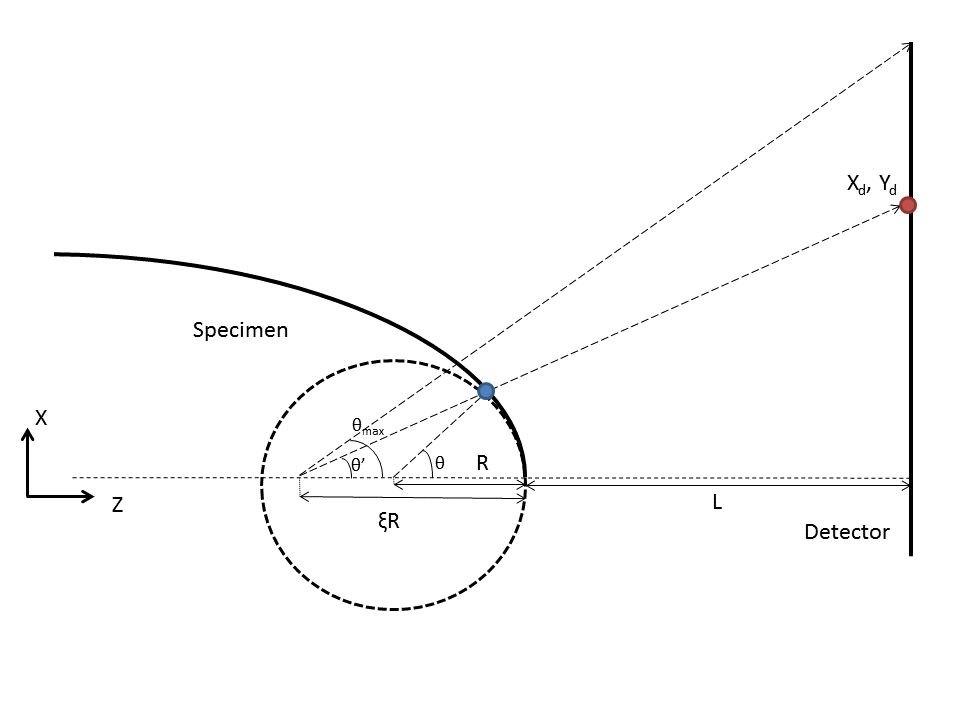
\includegraphics[width=\textwidth]{p3_projection}
	}
	\caption{Схематическое изображение точки-проекции: точка (X, Y) на наконечнике дает удар ($X_d$, $Y_d$). Определения углов в модели стереографической проекции.}
	\label{fig:p3_projection}
\end{figure} 
Координаты X и Y восстанавливаются с помощью стереографической проекции. Схема реконструкции представлена на Рисунке \cref{fig:p3_projection}. Прямая связь между двумя углами $\theta$ и $\theta$' и координатой Z может быть получена как:

\begin{equation}
	\label{eq:equation3_4}
	\theta = \theta' + \arcsin(\xi - 1)\sin{\theta'}
\end{equation}
\begin{equation}
	\label{eq:equation3_5}
	z_i = \frac{\Omega N_i}{Q R^2 \pi 2 {\sin^2(\theta_{max})}} + R (1- \cos{\theta})
\end{equation}

где $\theta$ - исходный угол запуска иона, который представляет собой реальный угол проекции, $\theta$' - угол, наблюдаемый после сжатия траекторий иона, Q - эффективность обнаружения, $N_i$ - номер обнаруженного атома. Угол $\theta_max$ - это максимальный угол обнаружения атомов. Уравнение \cref{eq:equation3_3} позволяет восстановить радиус в алгоритме Bas. Радиус впоследствии используется для восстановления координат. Важно отметить, что изменения kf играют важную роль в вычислении координаты Z, поскольку они влияют на значения обеих частей в сумме в \cref{eq:equation3_5}. Первая часть в \cref{eq:equation3_5} оказывает прямое влияние на координату Z. Второй (с ICF в $\theta$) - это поправка на кривизну поверхности. Следовательно, ICF влияет только на координаты X и Y. Чтобы продемонстрировать роль параметров реконструкции, одна и та же часть исследуемого образца была реконструирована с различными значениями $k_f$ и IFC (см. Рисунок \cref{fig:p3_3Dparts}). Как будет показано ниже, оптимальные значения $k_f$ и IFC могут быть выбраны, если реконструированная плотность материала образца приведена в соответствие с реальной.

\begin{figure}[htb]
	\centerfloat{
		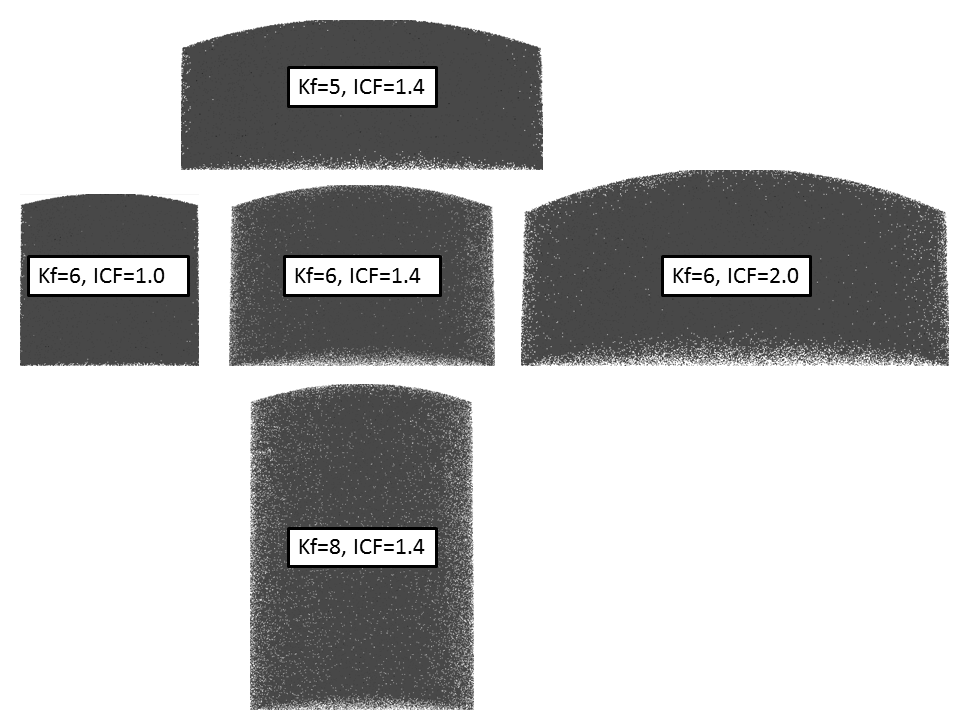
\includegraphics[width=\textwidth]{p3_3Dparts}
	}
	\caption{Карты атомов, построенные из одной и той же части исследуемого образца с различными параметрами $k_f$ и ICF}
	\label{fig:p3_3Dparts}
\end{figure}

\begin{figure}[htb]
	\begin{minipage}[b][][b]{0.49\textwidth}\centering
		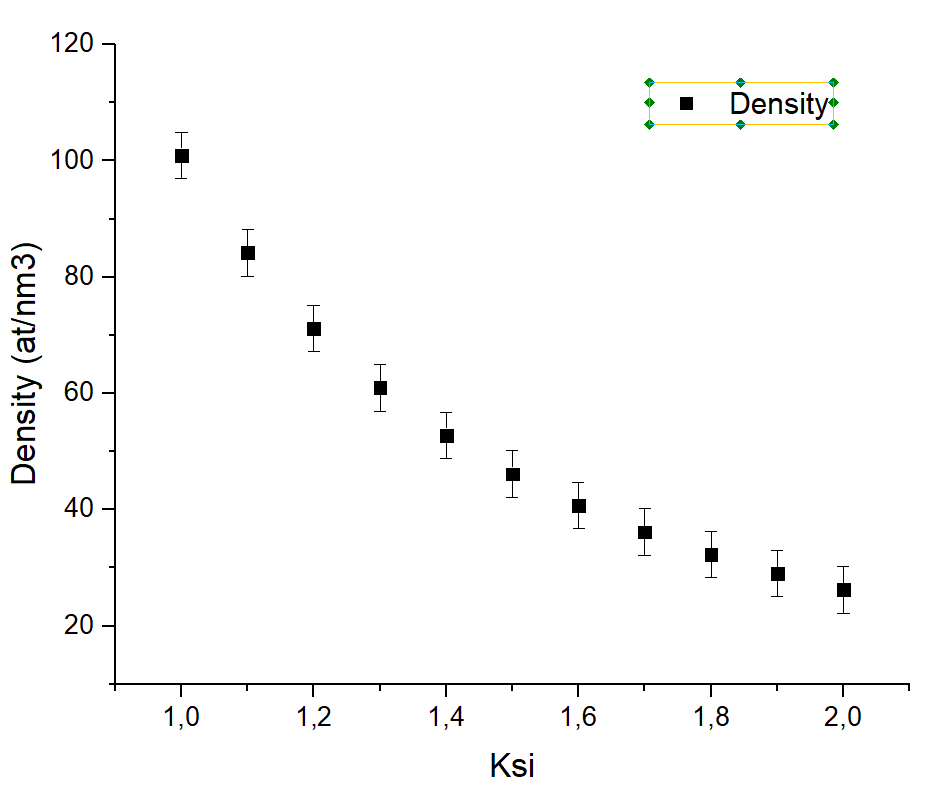
\includegraphics[width=\textwidth]{p3_ICFvsKsi} \\ а)
	\end{minipage}
	%\hfill
	\begin{minipage}[b][][b]{0.49\textwidth}\centering
		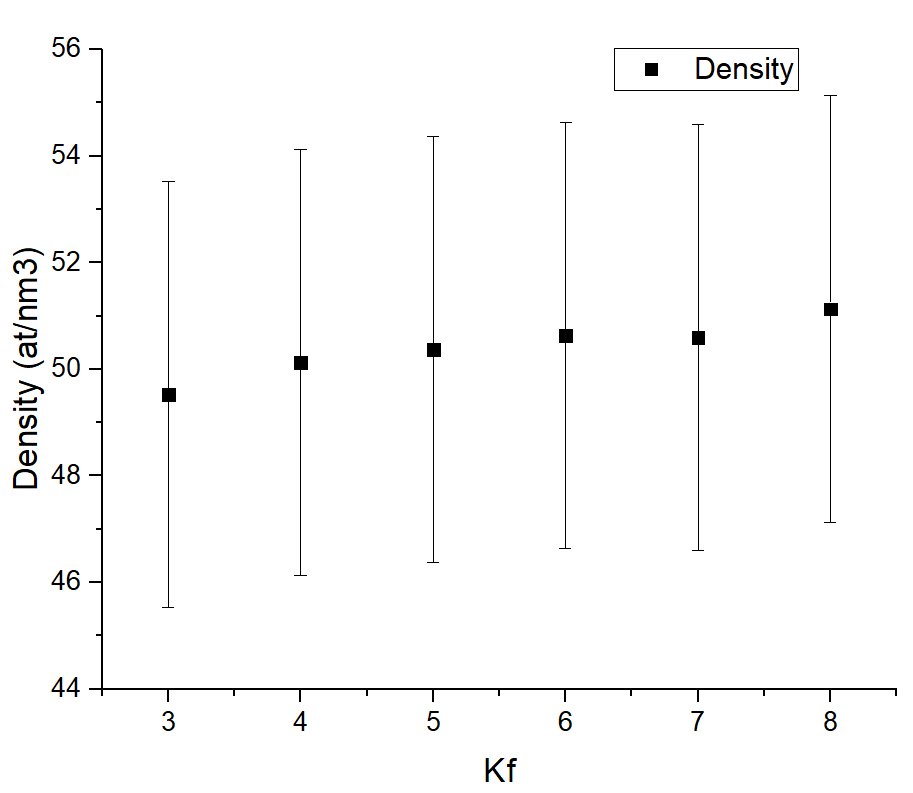
\includegraphics[width=\textwidth]{p3_ICFvskf} \\ б)
	\end{minipage}
	\caption{График атомной плотности как функции ICF (а). График атомной плотности как функции фактора поля $k_f$ (б)}
	\label{fig:p3_ICF}
\end{figure}

Следует отметить, что размер Z объема не изменяется при изменении ICF и фиксируется $k_f$, изменяются только радиус R и угол $\Theta$. Как объяснялось выше, это следствие выбранного алгоритма реконструкции. Как показано на Рисунке \cref{fig:p3_ICF} (б), атомная плотность не меняется с эволюцией $k_f$. Это связано с тем, что координаты X и Y пропорциональны радиусу, а Z обратно пропорциональна квадрату радиуса (см. Уравнения \cref{eq:equation3_1,eq:equation3_2,eq:equation3_5}). Таким образом, можно сделать вывод, что в алгоритме реконструкции $k_f$ и ICF можно откалибровать отдельно.
Принимая во внимание все перечисленные детали, предлагаем следующий алгоритм реконструкции. Первым шагом реконструкции является поиск динамического $k_f$. На значение $k_f$ напрямую влияет на все три координаты. Поэтому на данном этапе целесообразно использовать эмпирическую калибровку для восстановления кристаллических плоскостей. Второй шаг - это выбор динамического ICF, который практически не меняет расстояния в направлении Z. На этом этапе можно использовать плотность материала для определения правильной зависимости ICF. Мы предлагаем выбрать переменные параметры для согласования восстановленной плотности с реальной плотностью материала образца по всему объему.
Таким образом, при поиске ICF и $k_f$ используются известные значения, такие как межслоевые расстояния кристаллов и атомная плотность. Согласно работам групп Gault \cite{Gault11_Loi}, Loi \cite{Loi13} и Da Costa \cite{Hatzoglou19}, можно предположить, что зависимости ICF(U) и $k_f$(U), найденные для чистых материалов, будут одинаковыми по точности для сплавов.

Представленный АЗТ-анализ проводился на установке ПАЗЛ-3D в НИЦ Курчатовский институт - ИТЭФ \cite{scbibAPPLE}. В ПАЗЛ-3D используется лазерное полевое испарение, прямопролетная геометрия и программное обеспечение, разработанное в ИТЭФ. Образцы АЗТ получали электрохимическим методом с использованием стандартных электролитов. Форма кончика образцов контролировалась с помощью просвечивающего электронного микроскопа JEOL 1200 EX. В процессе сбора данных температура образца составляла 21 К, скорость сбора данных составляла от 2 до 6 атомов на 1000 лазерных импульсов, а энергия лазера составляла от 5 до 10 мВт с частотой 25 кГц. Для сплавов оптимальные условия испарения выбирались по методике, описанной в работе Разницына и др. \cite{scbibOptParamsYAFI}. Реконструкция данных проводилась с помощью программы КВАНТМ-3D \cite{KVANTM}. Для расчета масс-спектров с помощью этого программного обеспечения использовались процедуры автоматической калибровки и оптимизации \cite{Shutov19}.
Для восстановления массы и координат каждого атома использовалась программа КВАНТМ-3D. Для поиска зависимостей $k_f$(U) и ICF(U) были выбраны алюминий и вольфрам с гранецентрированной и объемноцентрированной кубической кристаллической структурой соответственно. Далее будут подробно описаны первый и второй этапы зависимостей поиска $k_f$(U) и ICF(U).

Как было написано выше, первым этапом алгоритма является поиск зависимости $k_f$ от напряжения на образце U. Объем образца разбивается на мелкие части по оси Z. Для каждой детали подбирается оптимальное расстояние между кристаллографическими плоскостями. Теоретические расстояния между атомными плоскостями соответствующих кристаллографических направлений взяты из приложения к книге Гаульта \cite{GaultBOOK}. Кристаллографические направления определялись по картам полевой десорбции. На Рисунке \cref{fig:p3_Alion} представлен пример карты полевой десорбции образца алюминия, полученной на АЗТ-детекторе.

\begin{figure}[htb]
	\centerfloat{
		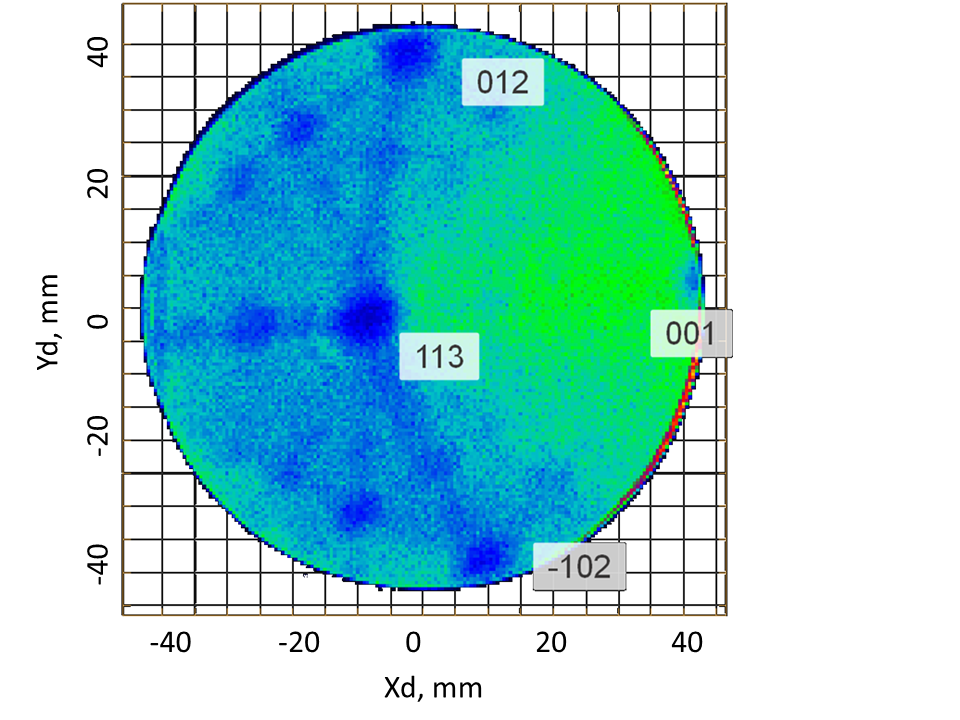
\includegraphics[width=\textwidth]{p3_Alion}
	}
	\caption{Карты полевой десорбции алюминиевого образца. Указаны кристаллографические направления}
	\label{fig:p3_Alion}
\end{figure} 

Для калибровки было выбрано ближайшее к центру детектора направление. Для большинства образцов этими направлениями были {111}, {001} и {113}. Информацию о межслоевых расстояниях, соответствующих выбранному направлению, можно взять из книги Гаульта \cite{GaultBOOK}. На Рисунке \cref{fig:p3_Alion} наиболее удобным направлением является {113} с расстоянием между атомными плоскостями около 1,2 \r{A}. Далее объем образца разбивался на мелкие части по оси Z. Каждая часть содержала 10-30 атомных плоскостей. Таким образом стало возможным найти значение $k_f$ для каждого небольшого кусочка образца. Напряжение на вершине в этих частях принималось постоянным для каждой из них. Полученные пары значений $k_f$ и напряжения U аппроксимировались функциональной зависимостью аналогичной в работе \cite{Hatzoglou19}. Пример аппроксимации данных выборки показан на Рисунке \cref{fig:p3_kf_vs_voltage}.

\begin{figure}[htb]
	\centerfloat{
		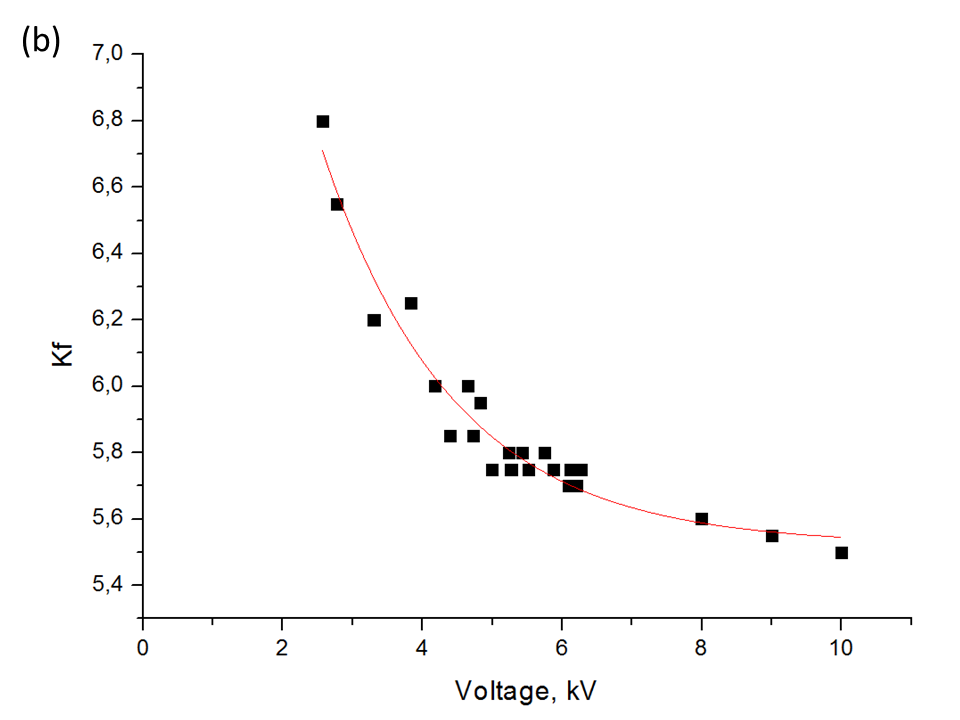
\includegraphics[width=\textwidth]{p3_kf_vs_voltage}
	}
	\caption{Экспериментальные данные $k_f$(черные точки) и наилучшая аппроксимирующая кривая (красная)}
	\label{fig:p3_kf_vs_voltage}
\end{figure} 

Описанная выше процедура была проведена для образцов из алюминия и вольфрама. $k_f$ как функция напряжения U была получена для каждой вершины. Из полученных данных была найдена общая зависимость $k_f$(U):

\begin{equation}
	\label{eq:equation3_6}
	k_f = (10 - C) + C\exp(- U * 5.3E-4)
\end{equation}

где C - константа подгонки. Значение постоянной зависит от состава материала. Например, для алюминия он равен 5,5, а для вольфрама - 4,5. Возможно, значение постоянной зависит от поля испарения материала. Явной разницы между коэффициентами в выражении \cref{eq:equation3_6} и углом стержня или начальным радиусом вершины не обнаружено. Полученная зависимость $k_f$(U) является экспоненциальной. Подобный характер зависимости был получен в работах Да Коста \cite{Hatzoglou19} и Лои \cite{Loi13}.
Следующим шагом после восстановления значения kf является корректировка значений ICF. Точность трехмерной реконструкции положения атомов в латеральном направлении недостаточна для идентификации кристаллической решетки. Согласно результатам, представленным на рис. 2, плотность может использоваться как критерий для получения значений ICF, обеспечивающих точность координат «сжатия» в плоскости XY. Тот же подход с разделением большого объема на мелкие части был использован для определения калибровочной кривой. Для каждой детали были найдены значение kf с использованием кристаллографических плоскостей и значение ICF с использованием плотности материала. Получена линейная зависимость ICF от напряжения на образце U. Зависимость ICF отличалась от полученных в аналогичных исследованиях \cite{Hatzoglou19, Gault11_Loi}. Это различие могло быть связано с режимом лазерного испарения в случае APPLE-3D в отличие от режима испарения с использованием локального электрода.
В программе анализа данных «КВАНТМ-3D» реализован инструмент «Линейная плотность» для построения графика атомной плотности вдоль выбранного направления. Атомная плотность рассчитывается вдоль выбранного направления. Для наглядности рисуется график с выбранным шагом. Примеры рассчитанных графиков плотности вдоль оси образца показаны на Рисунке \cref{fig:p3_Density_vs_depth} для алюминиевого образца с оптимизацией или без нее.

\begin{figure}[htb]
	\centerfloat{
		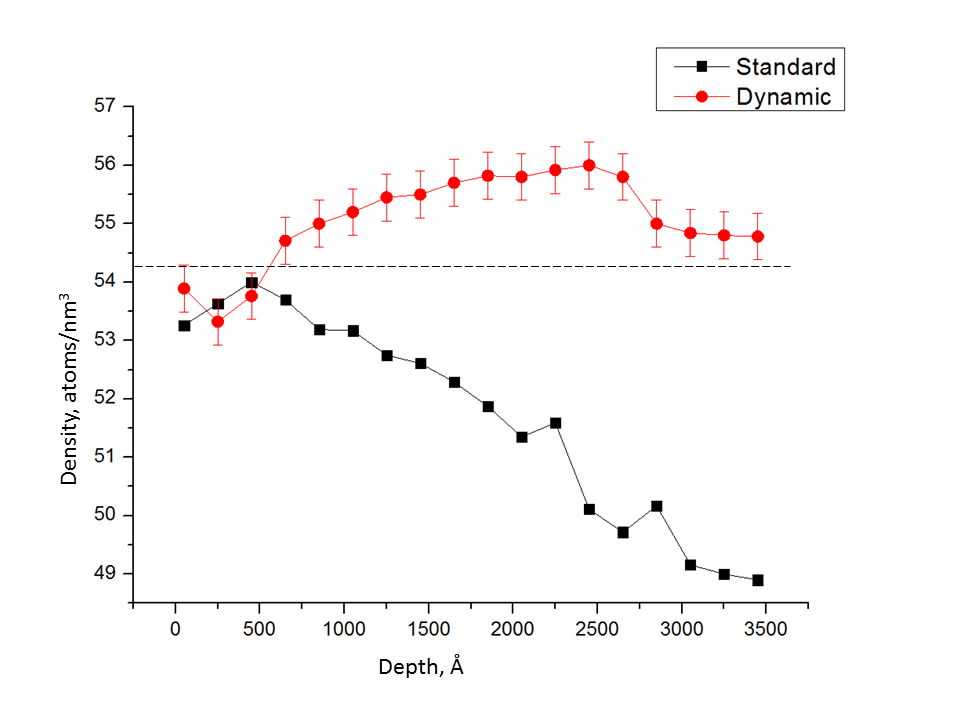
\includegraphics[width=\textwidth]{p3_Density_vs_depth}
	}
	\caption{Линейная атомная плотность вместе с образцом алюминия, полученная по стандартным протоколам и протоколам динамической реконструкции. Пунктирная линия показывает реальную плотность алюминия.}
	\label{fig:p3_Density_vs_depth}
\end{figure}

Необходимо скорректировать ожидаемую плотность для эффективности системы обнаружения для каждого прибора АЗТ, чтобы сравнить полученные значения с теоретическими. На использованной установке APPLE-3D установлена система детектирования с микроканальными пластинами с эффективностью детектирования ~ 90\%. В результате двух этапов калибровки были найдены динамические $k_f$ и ICF. Далее необходимо проверить эти зависимости на чистых материалах.

Предлагаемый протокол был протестирован на чистых материалах Al и W. Вольфрам имеет объемно-центрированную кубическую кристаллическую структуру с постоянной решетки около 3,16 \r{A} и 60,2 атома на кубический нанометр. Алюминий имеет гранецентрированную кубическую кристаллическую структуру с постоянной решетки около 4,05 \r{A} и 63,6 атома на кубический нанометр. Всего было исследовано 12 образцов алюминия и вольфрама. Для проверки точности реконструкции использовался специальный прибор для оценки расстояний между атомными плоскостями. Принцип этого инструмента основан на алгоритме распределения ближайших соседей k-го порядка \cite{GaultBOOK}. В программе КВАНТМ-3D этот инструмент называется «KNN-krist». Поиск соседей проводился только для атомов в выбранном направлении. Вместо дальнейшего поиска кластеров на гистограмму было нанесено распределение расстояний между ближайшими соседними атомами (см. Рисунок \cref{fig:p3_atomiccount_distance}). Расстояния между атомными плоскостями на разной глубине по оси Z были рассчитаны для всех образцов для стандартного и нового алгоритмов калибровки. Разница между этими алгоритмами показана на Рисунках \cref{fig:p3_PlanesDistance_depth,fig:p3_atomiccount_distance}.

\begin{figure}[htb]
	\centerfloat{
		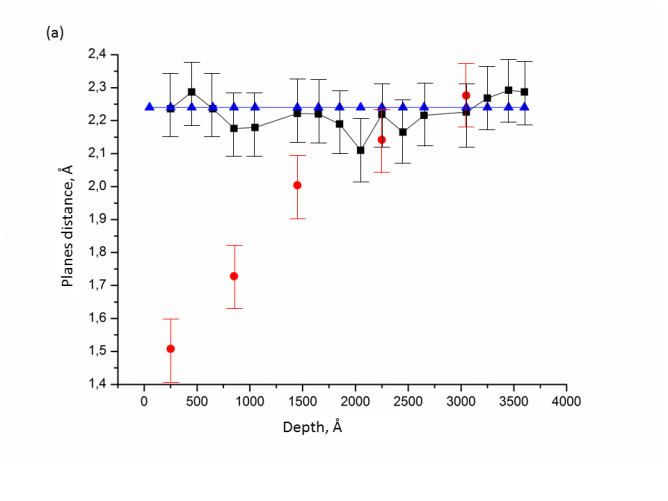
\includegraphics[width=\textwidth]{p3_PlanesDistance_depth}
	}
	\caption{Расстояние между атомными плоскостями как функция глубины по оси Z образца, полученное стандартным протоколом реконструкции (красный), динамическим протоколом $k_f$ и ICF (черный) и теоретическим значением (синий)}
	\label{fig:p3_PlanesDistance_depth}
\end{figure}
\begin{figure}[htb]
	\centerfloat{
		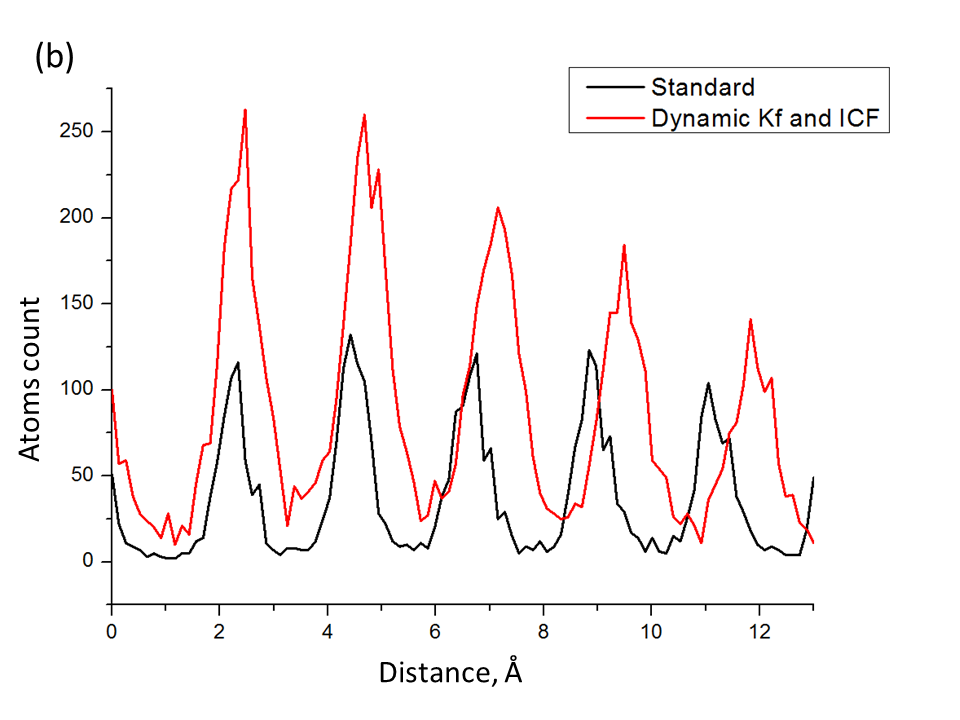
\includegraphics[width=\textwidth]{p3_atomiccount_distance}
	}
	\caption{Результат процедуры KNN-cryst для стандартных и динамических алгоритмов восстановления.}
	\label{fig:p3_atomiccount_distance}
\end{figure}

На Рисунке \cref{fig:p3_PlanesDistance_depth} видно, что ошибка в межплоскостных расстояниях, полученных в начале и в конце сбора данных АЗТ, может достигать 50\%. Важно отметить, что предлагаемые поправки могут значительно улучшить оценку размеров кластеров / фаз. Кроме того, учет этой поправки повлияет на точность расчета размеров переходных слоев, фаз и зерен. 
В этой статье был предложен алгоритм трехмерной реконструкции для данных АЗТ с использованием контроля плотности восстановленного материала. Этот протокол основан на алгоритме восстановления Баса. Отличительной особенностью этого протокола является проверка плотности материала вдоль выбранного направления для повышения точности восстановления данных. Динамические значения $k_f$ и ICF были измерены с использованием как кристаллографии, так и инструмента контроля плотности материала.

%\subsection{Подпараграф \cyrdash{} два}\label{subsec:ch3/sect33/sub2}

%Некоторый текст.

\clearpage
